% ===========================================================================
\section{Agricultural Air-Pollutant Co-emissions}
\label{sec:airpollutants}
% ===========================================================================

Agriculture is a major source of ammonia in South Asia. Crop-residue burning also produces
particulate matter and combustion gases that contribute to seasonal air-pollution episodes.

The air-pollutant inventory reports emissions in native mass units rather than converting
them to \COe{}. The calculation methods and nitrogen accounting are described in
Section~\ref{sec:methods-shared}; this section reports the resulting national, spatial,
historical and benchmark estimates.

The air-pollutant layer follows the same general processing framework as the greenhouse-gas
inventory. Emissions are calculated nationally and allocated to provinces, a
\SI{0.05}{\degree} grid and 116 districts using stream-specific spatial proxies. National
time series are reconstructed for 1990--2024, and parametric uncertainty is evaluated
analytically and by Monte-Carlo simulation.

The two layers differ in the status of their national totals. The greenhouse-gas total is
calculated within the formal IPCC inventory structure. The air-pollutant totals are bottom-up
estimates developed in this study. They therefore serve as separate control totals for the
air-pollutant spatial products and require external evaluation.

Each air-pollutant grid, district table and provincial allocation reproduces its
corresponding national pollutant total to a relative numerical residual below $10^{-9}$.

\subsection{National air-pollutant totals}

Agricultural \NHthree{} emissions in 2024 are estimated at \SI{2.67}{}~Mt.

Housing, yards and manure storage contribute approximately \SI{0.84}{}~Mt. Manure applied to
agricultural soils contributes a further \SI{0.87}{}~Mt. Synthetic fertiliser contributes
\SI{0.74}{}~Mt, and grazing deposition contributes approximately \SI{0.22}{}~Mt.
Crop-residue burning adds approximately \SI{9}{}~kt.

Crop-residue burning also produces an estimated \SI{654}{}~kt of CO, \SI{54}{}~kt of
PM$_{2.5}$, \SI{50}{}~kt of NMVOC, \SI{18}{}~kt of \NOx{}, \SI{3.6}{}~kt of black carbon and
\SI{2.8}{}~kt of SO$_2$. Agricultural soil processes contribute an additional \SI{145}{}~kt
of \NOx{}, bringing total agricultural \NOx{} emissions to approximately \SI{163}{}~kt.

Punjab contributes \SI{1.53}{}~Mt of \NHthree{}, followed by Sindh at \SI{0.61}{}~Mt, Khyber
Pakhtunkhwa at \SI{0.28}{}~Mt and Balochistan at \SI{0.26}{}~Mt.

The provincial pattern reflects the combination of fertilised cropland and livestock
production. Manure-application \NHthree{} is particularly sensitive to the spatial treatment
because it occurs neither strictly where manure is produced nor uniformly across cropland; it
is allocated using the intersection of livestock density and cropland.

\begin{table*}[!htbp]
\centering
\footnotesize
\begin{tabular}{@{}lrrrrrrr@{}}
\toprule
\textbf{Category (kt)} & \textbf{\NHthree{}} & \textbf{\NOx{}} & \textbf{PM$_{2.5}$}
& \textbf{CO} & \textbf{NMVOC} & \textbf{BC$^{a}$} & \textbf{SO$_2$} \\
\midrule
Managed soils      & 1822 & 145 & --- & --- & --- & --- & --- \\
Manure management  &  843 & --- & --- & --- & --- & --- & --- \\
Field burning      &    9 &  18 &  54 & 654 &  50 & 3.6 & 2.8 \\
\midrule
\textbf{Total}     & \textbf{2675} & \textbf{163} & \textbf{54} & \textbf{654}
& \textbf{50} & \textbf{3.6} & \textbf{2.8} \\
\bottomrule
\end{tabular}
\caption{Agricultural air-pollutant emissions in 2024, reported in kt of
native pollutant mass. Black carbon is included within PM$_{2.5}$ and should not be added to
it. \NOx{} is reported as NO$_2$-equivalent mass. The air-pollutant values define separate
national controls and are not components of the greenhouse-gas \COe{} total.
$^{a}$Black carbon is a \emph{component} of PM$_{2.5}$, not additive to
it. \NOx{} is reported as NO$_2$-equivalent mass. ``Managed soils''
\NHthree{} comprises synthetic fertiliser, manure applied to soils and grazing
deposition. Uncertainties are given per pollutant in Table~\ref{tab:apunc} and per
factor in Table~\ref{tab:apef}. Not part of the GHG control-total reconciliation.}
\label{tab:apresults}
\end{table*}

\subsection{Spatial distribution}
\label{sec:ap-spatial}

Each pollutant stream is allocated using the same dasymetric equation applied to the
greenhouse-gas inventory.

\NHthree{} from livestock housing, yards, storage and grazing follows gridded livestock
density. At district level, census head-counts replace the gridded proxy where suitable
matches are available.

\NHthree{} from manure application follows cropland weighted by livestock density.
Synthetic-fertiliser \NHthree{} follows cropland, with rice-specific nitrogen allocated to
mapped paddy area. Pollutants from residue burning follow satellite active-fire detections.

This common proxy framework keeps the greenhouse-gas and air-pollutant products spatially
consistent for nitrogen streams derived from the same activity.

Ammonia emissions are concentrated in the canal-belt and livestock-producing districts.
Jhang has the highest district estimate at approximately \SI{93}{}~kt, followed by
Muzaffargarh at \SI{85}{}~kt, Sheikhupura at \SI{83}{}~kt, Sargodha at \SI{75}{}~kt and
Rahim Yar Khan at \SI{66}{}~kt.

Karachi---the one polygon that receives the division's seven census districts, Malir's
peri-urban dairy colonies the largest part---again represents a livestock-dominated profile,
whereas the leading Punjab districts combine livestock and intensive cultivation.

\begin{figure}[!htbp]
\centering
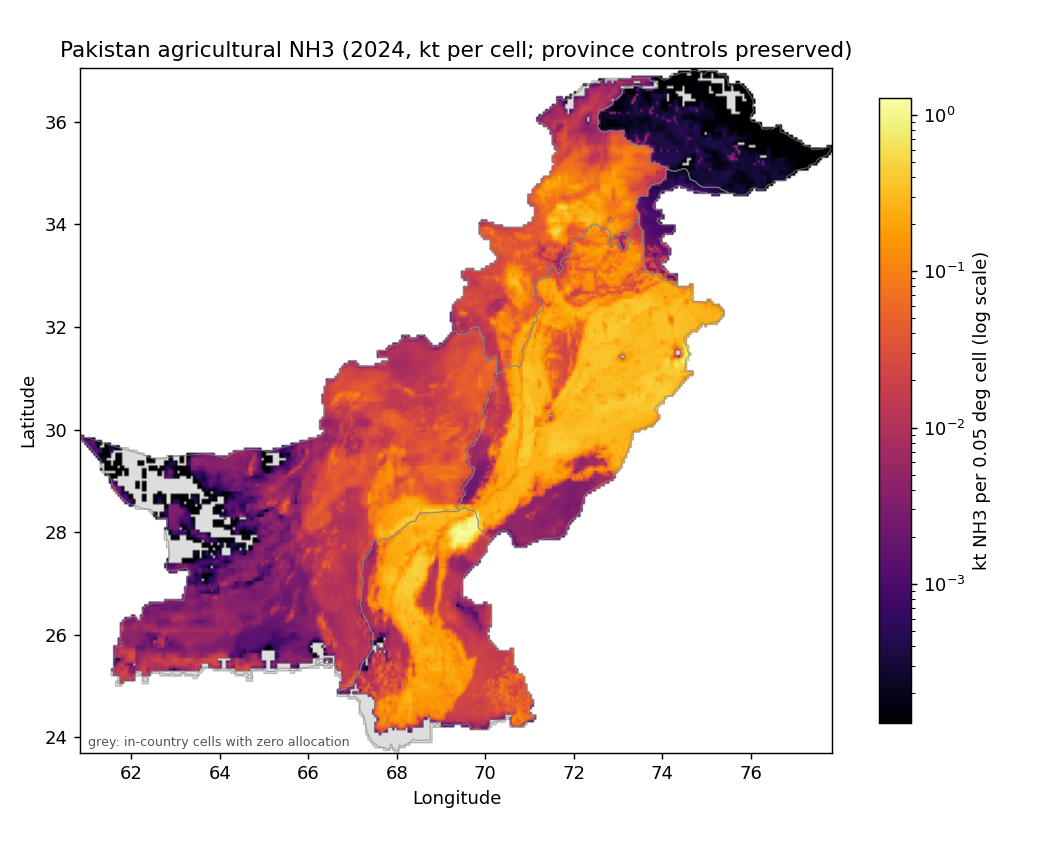
\includegraphics[width=\linewidth]{nh3_map.png}
\caption{Agricultural \NHthree{} emissions on the \SI{0.05}{\degree} grid in
2024, reported as kt \NHthree{} per cell on a logarithmic scale. Each nitrogen stream is
allocated using its process-specific spatial proxy, and the combined surface reproduces the
provincial and national air-pollutant totals.}
\label{fig:nh3map}
\end{figure}

\subsection{Historical trajectory}
\label{sec:ap-timeseries}

Agricultural \NHthree{} emissions increase from approximately \SI{784}{}~kt in 1990 to
\SI{2675}{}~kt in 2024, a factor of \num{3.4}.

The increase reflects growth in livestock populations and synthetic-fertiliser use. Emission
factors remain fixed throughout the series, so changes represent the historical activity
data.

CO from crop-residue burning increases from approximately \SI{250}{}~kt to \SI{654}{}~kt, a
factor of \num{2.6}. The remaining crop-burning pollutants follow the same underlying change
in burned dry matter.

As in the greenhouse-gas reconstruction, the 1990--2023 estimates use FAOSTAT activity data,
while 2024 is anchored to the PBS census and current Pakistani statistics. The difference in
crop coverage at this transition is discussed in Section~\ref{sec:limitations}.

\begin{figure}[!htbp]
\centering
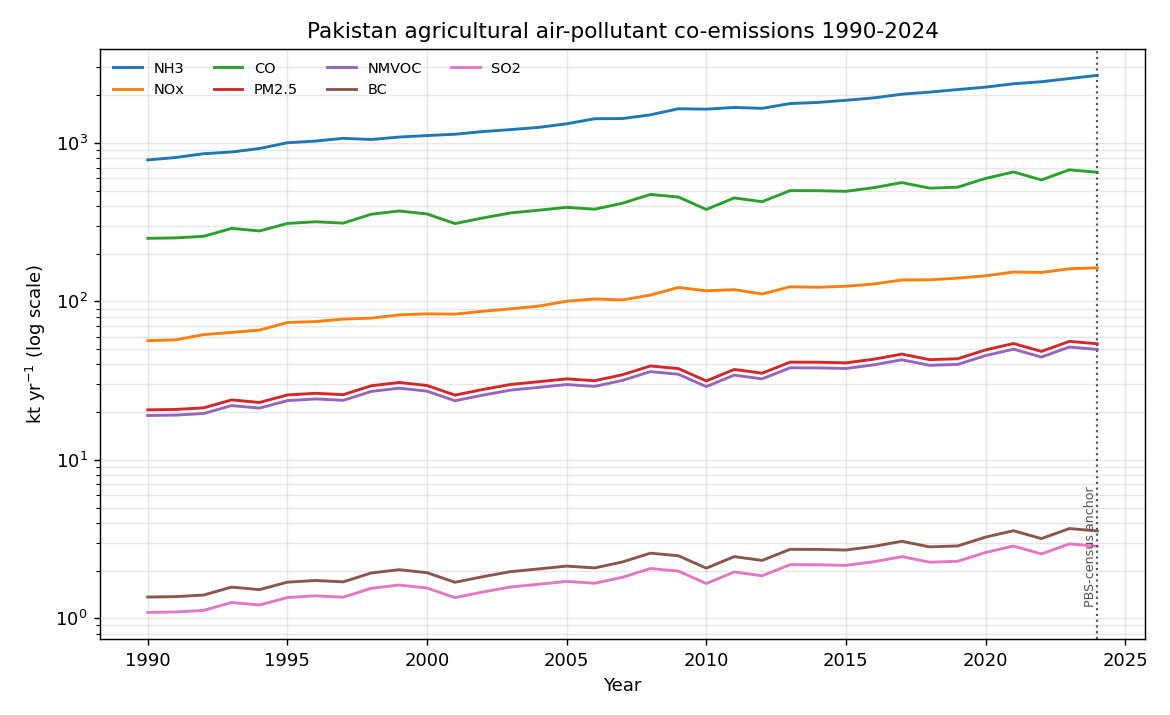
\includegraphics[width=\linewidth]{air_trend.png}
\caption{Agricultural air-pollutant emissions, 1990--2024, reported in kt on a
logarithmic scale. The vertical marker identifies the 2024 transition from the FAOSTAT
activity series to the PBS census anchor.}
\label{fig:airtrend}
\end{figure}

\subsection{Parametric uncertainty and key sources}

Air-pollutant uncertainty is propagated using the same analytical and Monte-Carlo procedures
as the greenhouse-gas inventory.

The Monte-Carlo analysis gives a mean \NHthree{} estimate of \SI{2676}{}~kt and a
\SI{95}{\percent} interval of \SI{2120}{}--\SI{3359}{}~kt. The corresponding Approach~1
relative half-width is $\pm$24\%.

Among the reported pollutants, \NHthree{} has the narrowest parametric relative interval.
Soil and fertiliser \NOx{} have the widest combined uncertainty at $\pm$90\%. Crop-burning
uncertainties range from $\pm$54\% for CO to $\pm$79\% for SO$_2$.

The comparatively narrow \NHthree{} parametric interval does not include uncertainty in the
national manure-management distribution. That structural uncertainty is evaluated separately
in Section~\ref{sec:ap-structural}.

Four sources qualify as key for \NHthree{}: manure applied to soils, contributing
approximately \SI{32}{\percent}; livestock housing and storage, contributing
\SI{32}{\percent}; synthetic fertiliser, contributing \SI{28}{\percent}; and small-ruminant
grazing, contributing \SI{4}{\percent}. Together these sources exceed the cumulative
\SI{95}{\percent} threshold. The \emph{ordering} of the three leading sources is soft, and
the published ranking now says so quantitatively: under the per-source Monte Carlo their
level shares overlap almost completely (each spanning roughly 20--44\%), and each holds its
point-estimate rank in only about a third to a half of draws
(\texttt{rank\_stability\_pct} in \texttt{outputs/air\_key\_categories.csv}). The key-source
\emph{set} is stable; which of the three leads is not resolvable at the current
uncertainties. Each of the remaining pollutants is dominated by crop-residue burning, so
residue burning is its principal key source---at \SI{100}{\percent} of the pollutant's
total, a statement about coverage (no other stream is estimated) rather than certainty,
as the table's note column records.

\begin{table*}[!htbp]
\centering
\footnotesize
\begin{tabular}{@{}lrrrrr@{}}
\toprule
\textbf{Pollutant} & \textbf{Mean} & \textbf{P2.5} & \textbf{P50} & \textbf{P97.5}
& \textbf{$\pm$\%} \\
\midrule
\NHthree{}   & 2676 & 2120 & 2657 & 3359 & 23 \\
\NOx{}       &  163 &   67 &  148 &  349 & 90 \\
CO           &  653 &  376 &  628 & 1074 & 54 \\
PM$_{2.5}$   &   54 &   28 &   52 &   94 & 62 \\
NMVOC        &   50 &   24 &   47 &   93 & 70 \\
BC           &  3.5 &  1.7 &  3.4 &  6.6 & 70 \\
SO$_2$       &  2.8 &  1.2 &  2.6 &  5.6 & 79 \\
\bottomrule
\end{tabular}
\caption{Monte-Carlo means and \SI{95}{\percent} intervals for agricultural air
pollutants, together with IPCC Approach~1 relative half-widths. The estimates include
parameter and activity-data uncertainty under the reference manure-management configuration
but exclude structural uncertainty among alternative management configurations.}
\label{tab:apunc}
\end{table*}

\subsection{Inventory scope and completeness}
\label{sec:ap-completeness}

The air-pollutant inventory distinguishes estimated sources, known unestimated sources, and
sources outside the agricultural activity basis. Three reporting conventions are important.

First, black carbon is a component of PM$_{2.5}$ and must not be added to the PM$_{2.5}$
estimate. Second, \NOx{} is reported as NO$_2$-equivalent mass, a convention that differs
from the underlying nitrogen or NO mass used in parts of the calculation. Third, the
inventory estimates emissions. It does not estimate ambient concentrations, population
exposure or health effects, and no atmospheric transport or chemistry model is applied in
this study.

Agricultural machinery and tillage or harvest dust are the main declared source gaps.
Suitable activity data and methods for these sources are not included in the present system.

\begin{table*}[!htbp]
\centering
\footnotesize
\begin{tabular}{@{}lccccccc@{}}
\toprule
\textbf{Source} & \textbf{\NHthree{}} & \textbf{\NOx{}} & \textbf{PM$_{2.5}$}
& \textbf{PM$_{10}$} & \textbf{CO} & \textbf{NMVOC} & \textbf{SO$_2$} \\
\midrule
Livestock housing and storage & E  & NE & NE & NE & --- & NE & --- \\
Grazing deposition            & E  & NE & --- & --- & --- & --- & --- \\
Manure application            & E  & E$^{a}$ & --- & --- & --- & --- & --- \\
Synthetic fertiliser          & E  & E  & --- & --- & --- & --- & --- \\
Residues left in field        & E$^{b}$ & NE & --- & --- & --- & --- & --- \\
Residue burning               & E  & E  & E  & NE & E  & E  & E \\
Agricultural machinery        & NE & NE & NE & NE & NE & NE & NE \\
Tillage and harvest dust      & --- & --- & NE & NE & --- & --- & --- \\
\bottomrule
\end{tabular}
\caption{Completeness assessment for agricultural air pollutants.
``Estimated'' indicates sources quantified in this inventory, ``not estimated'' identifies
known sources outside the current calculation, and a dash indicates that the
source--pollutant combination is not applicable. Black carbon is included within
PM$_{2.5}$.
$^{a}$Included in the soil \NOx{} term, which is parameterised on total
applied nitrogen rather than per source. $^{b}$Estimated as a computed zero
(Section~\ref{sec:ap-scope}). Black carbon (estimated for residue burning) is a component of
PM$_{2.5}$, not additive to it. Agricultural machinery and tillage dust are outside this
inventory's activity basis and are the largest declared gaps.}
\label{tab:apcompleteness}
\end{table*}

\subsection{Spatial-proxy crosswalk}
\label{sec:ap-crosswalk}

Table~\ref{tab:crosswalk} summarises the spatial proxy used for each emission stream at
provincial, gridded and district levels.

Livestock housing and storage use livestock shares at provincial level, \GLW{} density on the
grid, and PBS census head-counts at district level. Grazing uses the same broad livestock
basis, with species distinctions retained where relevant.

Applied manure uses the cropland--livestock intersection. Synthetic fertiliser uses provincial
offtake, cropland on the grid, and district cropland, except for the rice-specific stream,
which uses rice area at each scale.

Crop residues retained in fields use crop production and cropland proxies. Residue-burning
pollutants use crop production for provincial controls and FIRMS active-fire detections for
grid and district allocation.

Using one crosswalk for the greenhouse-gas and air-pollutant modules prevents corresponding
nitrogen streams from being assigned incompatible spatial proxies.

\begin{table*}[!htbp]
\centering
\footnotesize
\begin{tabular}{@{}llll@{}}
\toprule
\textbf{Emission stream} & \textbf{Province} & \textbf{Grid} & \textbf{District} \\
\midrule
Housing/storage \NHthree{}, manure \CHfour{}/\NtwoO{} & livestock & \GLW{} density & PBS census heads \\
Grazing \NHthree{}, pasture \NtwoO{} & livestock (small rum.\ split) & \GLW{} density & PBS census heads \\
Applied-manure \NHthree{}/\NtwoO{} & manure-applied & cropland $\times$ \GLW{} & census $\times$ cropland \\
Synthetic fertiliser, upland & fertiliser offtake & cropland & district cropland \\
Synthetic fertiliser, rice & rice area & MapSPAM rice (held, hash-pinned) & official rice area \\
Crop residues (returned) & crop production & cropland & district cropland \\
Residue burning, all pollutants & crop production & FIRMS active fire & FIRMS active fire \\
Urea \COtwo{} & fertiliser offtake & cropland & district cropland \\
\bottomrule
\end{tabular}
\caption{Spatial proxies used for greenhouse-gas and air-pollutant emission
streams at provincial, gridded and district levels. Corresponding nitrogen streams use a
shared proxy lookup in both inventory layers.}
\label{tab:crosswalk}
\end{table*}

\subsection{Structural uncertainty in manure management}
\label{sec:ap-structural}

The $\pm$24\% parametric uncertainty for \NHthree{} holds the assumed distribution of
manure-management systems constant. That distribution is itself poorly constrained.

No national survey measures how excreted nitrogen in Pakistan is divided among grazing,
confined manure systems and dung used as fuel. Available regional and external
parameterisations imply substantially different distributions.

Four configurations were evaluated using the same calculation framework.

The reference configuration is consistent with the FAOSTAT-based manure-management
assumptions used in the greenhouse-gas inventory. It assigns \SI{41}{\percent} of excreted
nitrogen to grazing and produces \SI{2.67}{}~Mt \NHthree{}. Livestock sources account for
\SI{1.93}{}~Mt of this total, and the corresponding agricultural greenhouse-gas total under
the evaluation harness's own re-implementation is \SI{223.5}{}~Mt~\COe{}
(Table~\ref{tab:apstruct}); the inventory's reference total is \SI{223.5}{}~Mt~\COe{}
(Section~\ref{sec:results}), and the harness figure is never used as a headline.

A benchmark-like configuration assigns \SI{70}{\percent} of excreted nitrogen to grazing. It
produces \SI{1.67}{}~Mt \NHthree{} and a greenhouse-gas total of \SI{217.7}{}~Mt~\COe{}.

The GLEAM~3.0 South Asia configuration \citep{gleam2022} assigns \SI{31}{\percent} to
grazing. It produces \SI{3.05}{}~Mt \NHthree{} and a greenhouse-gas total of
\SI{233.4}{}~Mt~\COe{}.

A midpoint diagnostic gives \SI{2.46}{}~Mt \NHthree{} and \SI{224.8}{}~Mt~\COe{}. This
midpoint is provided only for orientation. It is not evidence-weighted, and the available
configurations are not independent observations.

Across the defensible configurations, national \NHthree{} ranges from \SI{1.67}{} to
\SI{3.05}{}~Mt, and the agricultural greenhouse-gas total varies by approximately
\SI{16}{}~Mt~\COe{}.

The structural and parametric uncertainties are reported separately. The management
configurations are discrete methodological alternatives rather than draws from a known
probability distribution, so combining them into one conventional confidence interval would
require unsupported assumptions about their likelihood.

The \SI{2.67}{}~Mt value should therefore be interpreted as the reference-configuration
estimate. It is used because it keeps the greenhouse-gas and air-pollutant calculations on a
common set of management assumptions, not because national evidence demonstrates that this
configuration is more probable than the alternatives.

\begin{table}[!htbp]
\centering
\footnotesize
\setlength{\tabcolsep}{4pt}
\begin{tabular}{@{}p{0.34\linewidth}rrrr@{}}
\toprule
\textbf{Management configuration} & \textbf{Grazing} & \textbf{\NHthree{}}
& \textbf{Livestock} & \textbf{GHG total} \\
 & \textbf{share} & \textbf{(Mt)} & \textbf{\NHthree{} (Mt)} & \textbf{(Mt \COe)} \\
\midrule
Current (FAOSTAT-consistent)  & 0.41 & 2.67 & 1.93 & 223.5 \\
Benchmark-like (high grazing) & 0.69 & 1.67 & 0.92 & 217.7 \\
GLEAM 3.0 South Asia$^{a}$    & 0.32 & 3.05 & 2.30 & 233.4 \\
Midpoint diagnostic$^{b}$     & 0.47 & 2.46 & 1.72 & 224.8 \\
\bottomrule
\end{tabular}
\caption{Sensitivity of national \NHthree{} and greenhouse-gas emissions to
alternative manure-management distributions. The reference case follows the assumptions used
in the main greenhouse-gas inventory. The midpoint is an unweighted diagnostic and should not
be interpreted as a preferred estimate.
$^{a}$\citet{gleam2022}.
$^{b}$An unweighted mean of the three configurations, carried as a midpoint for orientation
only. It is not evidence-weighted: the three are not independent and no defensible weighting
exists, so it should not be read as a best estimate.
Generated by \texttt{src/pkinv/eval/mms\_structural\_uncertainty.py}.}
\label{tab:apstruct}
\end{table}

\subsection{Allocation assumptions and residue-derived ammonia}
\label{sec:ap-scope}

\paragraph{Manure application}
The spatial distribution of manure-application \NHthree{} is based on a process-informed
proxy rather than direct observation.

Livestock density alone would place the emission where manure is generated, including
rangelands where little manure is applied to crops. Cropland alone would distribute manure
independently of nearby livestock supply and transport constraints. The adopted proxy weights
cropland by livestock density at the grid-cell level, and therefore identifies cultivated land
located close to manure production.

This treatment produces plausible differences among provinces. Sindh receives a relatively
high share because intensive cropland and livestock occupy the same Indus corridor.
Balochistan receives a lower share because much of its livestock population is located in
extensive rangelands with little adjacent cropland.

The proxy does not represent actual hauling distances or manure markets. A national or
regional survey of manure transport and application would provide a stronger empirical basis.

\paragraph{Crop residues left in fields}
\NHthree{} from residues left to decompose in fields is estimated as zero rather than
omitted.

The adopted EMEP/EEA method produces net \NHthree{} only when the nitrogen content of the
residue exceeds \num{0.0132}. Below this threshold, microbial immobilisation offsets the
ammonia that would otherwise be released.

All crops represented in the inventory fall below the threshold. Cotton is closest at
\num{0.0120}. Rice is \num{0.0070}, wheat and maize are \num{0.0060}, and sugarcane is
\num{0.0040}.

A sensitivity test raises all residue nitrogen contents by \SI{50}{\percent}. Under this
test cotton exceeds the threshold, but the resulting national emission is only
\SI{0.03}{}~kt \NHthree{}. The calculated zero is therefore sensitive to the formal
threshold, but the national consequence is negligible.

The external South Asian inventory reports approximately \SI{1.4}{}~kt for this stream using
a wider crop set. This difference accounts for only about \SI{0.1}{\percent} of its national
agricultural \NHthree{} total and does not explain the broader benchmark difference.

\subsection{External spatial comparison}

The \SI{0.05}{\degree} \NHthree{} surface is compared with the independent \SI{0.1}{\degree}
South Asian agricultural ammonia inventory for 2015 \citep{sanh2026data}.

Our inventory is recalculated using 2015 activity and aggregated exactly from
\SI{0.05}{\degree} to the benchmark's \SI{0.1}{\degree} grid. The comparison covers
\num{8322} grid cells within Pakistan.

Before calculating spatial statistics, the benchmark grid is summed over the national mask.
The resulting total is \SI{1052}{}~kt, compared with \SI{1043}{}~kt in the benchmark's
published national table. The difference is below \SI{1}{\percent}, supporting the grid
interpretation, unit conversion and national mask.

At aggregate level the two surfaces show strong spatial agreement: Pearson $r=0.90$, Spearman
$\rho=0.90$, log-space Pearson $r=0.74$, and \SI{78}{\percent} overlap among top-decile
cells.

Despite this spatial agreement, our national 2015 total is \num{1.76} times the gridded
benchmark value. The ratio is similar across Punjab, Sindh and Khyber Pakhtunkhwa, at
approximately \num{1.72}--\num{1.77}. This indicates that most of the difference is in
national magnitude rather than in broad spatial distribution.

Balochistan is an exception, with a ratio of \num{2.78}. Its \NHthree{} estimate is dominated
by extensive livestock systems, making it particularly sensitive to the uncertain division
between grazing and managed manure systems.

The aggregate spatial correlation partly reflects shared inputs. Both inventories allocate
livestock emissions using \GLW{}, and livestock accounts for most agricultural \NHthree{}.
The stream-level comparison is therefore more informative.

Synthetic-fertiliser emissions use different underlying crop surfaces in the two inventories.
This stream agrees in both pattern and magnitude, with $r=0.89$, \SI{72}{\percent} top-decile
overlap and a level ratio of \num{1.19}.

Residue-burning \NHthree{} also uses different surfaces. Agreement is weak, with $r=0.38$,
\SI{39}{\percent} top-decile overlap and a level ratio of \num{0.21}.

The comparison therefore supports the fertiliser allocation most strongly. It shows that the
livestock difference is mainly one of magnitude, while the burning stream differs in both
pattern and level.

Two qualifications remain. The inventory uses fixed-vintage within-province spatial proxies,
so changes between 2015 and 2024 arise from provincial controls rather than from evolving
internal patterns. In addition, the sector definitions of the two inventories are similar but
not identical.

\begin{figure}[!htbp]
\centering
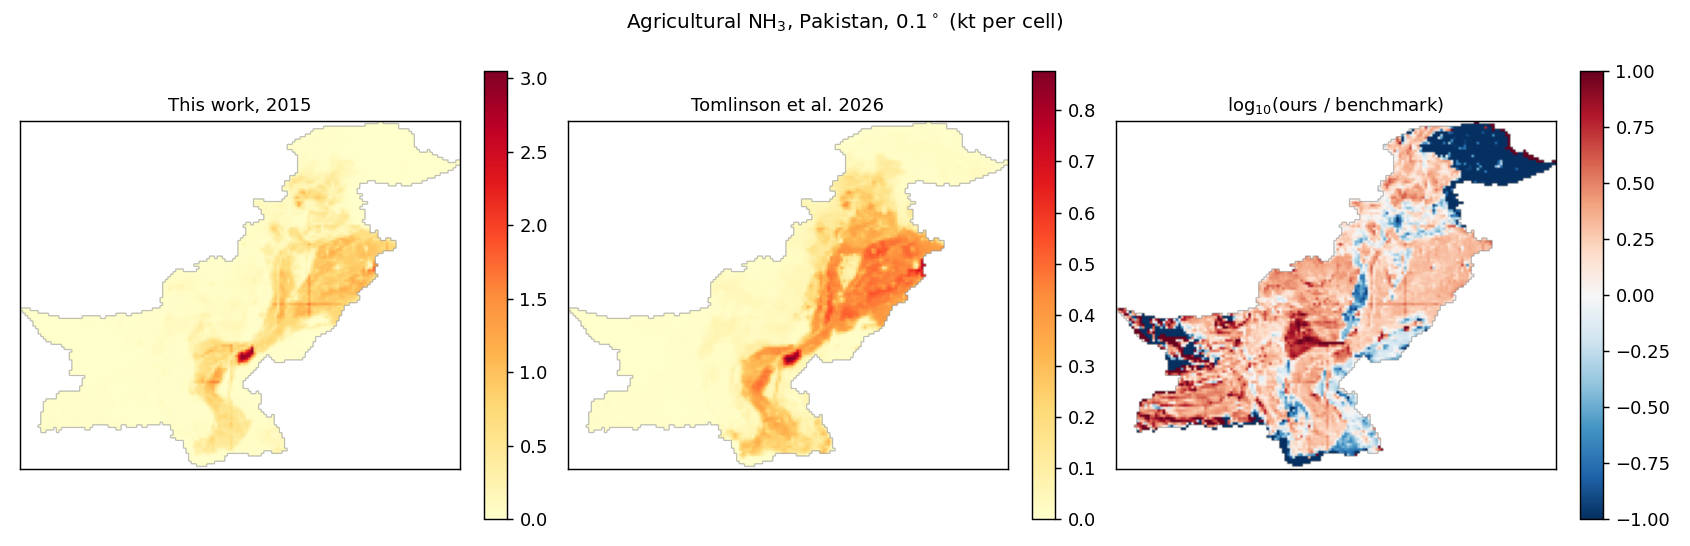
\includegraphics[width=\linewidth]{nh3_spatial_comparison.png}
\caption{Agricultural \NHthree{} emissions over Pakistan in 2015 at
\SI{0.1}{\degree} resolution: this inventory, the independent South Asian benchmark, and their
ratio. The two surfaces show strong spatial agreement but differ in magnitude, with the
largest relative difference over Balochistan's rangelands.
Generated by
\texttt{src/pkinv/eval/spatial\_nh3\_validation.py}.}
\label{fig:nh3spatial}
\end{figure}

\begin{table*}[!htbp]
\centering
\footnotesize
\begin{tabular}{@{}llrrrc@{}}
\toprule
\textbf{Stream} & \textbf{Our spatial input} & \textbf{$r$} & \textbf{Hotspot} & \textbf{Ratio}
& \textbf{Shared?} \\
\midrule
Synthetic fertiliser & WorldCover (upland; rice on MapSPAM) & 0.89 & 72\% & 1.19 & no \\
Livestock (all)      & \GLW{}             & 0.91 & 78\% & 2.47 & \textbf{yes} \\
Residue burning      & FIRMS active fire   & 0.38 & 39\% & 0.21 & no \\
\midrule
All streams          & ---                 & 0.90 & 78\% & 1.76 & partly \\
\bottomrule
\end{tabular}
\caption{Stream-level spatial comparison with the independent South
Asian agricultural \NHthree{} inventory for 2015. The livestock comparison uses a shared
\GLW{} spatial product and is therefore not fully independent. Fertiliser and residue-burning
comparisons use different spatial inputs in the two inventories.
Generated by
\texttt{src/pkinv/eval/spatial\_nh3\_validation.py}.}
\label{tab:spatialstreams}
\end{table*}

\subsection{Comparison of national ammonia estimates}
\label{sec:ap-benchmark}

National \NHthree{} is compared with the South Asian benchmark at the benchmark year of 2015.

Matching the comparison year is important. Agricultural \NHthree{} in the present
reconstruction increases by a factor of \num{1.44} between 2015 and 2024. Comparing the
benchmark's 2015 value directly with the 2024 anchor would combine methodological differences
with nine years of activity growth.

For 2015 this inventory estimates \SI{1862}{}~kt \NHthree{}, compared with \SI{1043}{}~kt in
the South Asian benchmark \citep{sanh2026}. The ratio is \num{1.79}. Comparing the same
benchmark with the 2024 estimate would produce a ratio of \num{2.56}. The 2015 estimate is
\num{1.48} times the corresponding EDGAR v8 value and \num{1.36} times the HTAP v3 value.

The uncertainty intervals provide a stronger diagnostic than the operational factor-of-two
screening range. The South Asian benchmark reports a \SI{95}{\percent} interval of
approximately \SI{764}{}--\SI{1322}{}~kt for Pakistan. The present inventory's 2015 interval
is approximately \SI{1423}{}--\SI{2307}{}~kt. The intervals do not overlap, and the
uncertainty-normalised difference is $z=3.1$. The national difference is therefore larger
than the parametric uncertainty reported by either inventory.

Agreement varies sharply by source. Synthetic-fertiliser \NHthree{} is \num{1.20} times the
benchmark value. Livestock \NHthree{} is approximately \num{2.50} times the benchmark.
Residue-burning \NHthree{} is \num{0.22} times the benchmark value.

The shared nitrogen ledger helps diagnose the livestock difference. After conversion to common
boundaries and an \NHthree{}-N basis, the IPCC and EMEP/EEA livestock chains produce totals
that differ by only a factor of \num{1.24}. However, both remain substantially above the
external benchmark.

This suggests that the difference cannot be attributed solely to choosing the IPCC or
EMEP/EEA loss formulation. Their stage-level estimates remain different, so the formulation
may still contribute, but the shared excreted-nitrogen pool and the assumed
manure-management distribution also require examination.

Country-specific animal masses increase estimated nitrogen excretion. Buffalo are assigned a
typical mass of \SI{380}{\kilogram}, compared with the IPCC default of \SI{295}{\kilogram},
while dairy cattle are assigned \SI{400}{\kilogram} rather than \SI{275}{\kilogram}. The
greenhouse-gas inventory shows a related signal: manure-management emissions are \num{1.38}
times the FAOSTAT value.

The external benchmark does not report an implicit emission factor for buffalo, despite
buffalo being a major component of Pakistan's livestock population. A residual calculation
based on its published national total and the species it reports implies a buffalo factor no
greater than approximately \SI{3.9}{}~kg \NHthree{} per head per year, as set out in
Supplementary Note~S4.

The present reference configuration gives approximately \SI{9.8}{}~kg per buffalo per year,
and the GLEAM~3.0 configuration gives \SI{11.7}{}~kg per head per year. These external
parameterisations therefore imply markedly different assumptions about the treatment of
buffalo manure, particularly the proportion deposited during grazing.

The inferred benchmark factor is not a direct observation. It is calculated as a residual and
also absorbs unresolved contributions from camels. It should therefore be treated as an
indication of where the discrepancy may arise rather than as a definitive attribution.

The available evidence points most strongly to the manure-management distribution, with
animal-mass assumptions and stage-specific loss formulations as additional contributors.
Because the manure-management distribution has not been measured nationally, the livestock
\NHthree{} estimate remains provisional.

The lower residue-burning estimate reflects the wider set of burned crops included in the
external inventory. Its additional \SI{1.4}{}~kt estimate for residues left in fields is too
small to explain the national difference and would increase rather than reduce the gap.

\begin{table*}[!htbp]
\centering
\footnotesize
\begin{tabular}{@{}llrrcrc@{}}
\toprule
& & & \multicolumn{2}{c}{\textbf{Matched year (2015)}}
& \multicolumn{2}{c}{\textbf{Anchor (2024)}} \\
\cmidrule(lr){4-5}\cmidrule(lr){6-7}
\textbf{Scope} & \textbf{Benchmark} & \textbf{Bench.}
& \textbf{Engine} & \textbf{Ratio} & \textbf{Engine} & \textbf{Ratio} \\
\midrule
Synthetic fertiliser & SANH 2026 & 514 & 617 & 1.20 & 737 & 1.43 \\
Livestock (all streams) & SANH 2026 & 496 & 1238 & 2.50$^{\dagger}$ & 1928 & 3.89$^{\dagger}$ \\
Residue burning & SANH 2026 & 32 & 7.0 & 0.22$^{\dagger}$ & 9.2 & 0.29$^{\dagger}$ \\
\midrule
\textbf{National total} & SANH 2026 & 1043 & 1862 & \textbf{1.79} & 2674 & 2.56$^{\dagger}$ \\
\textbf{National total} & EDGAR v8$^{a}$ & 1257 & 1862 & \textbf{1.48} & 2674 & 2.13$^{\dagger}$ \\
\textbf{National total} & HTAP v3$^{a}$ & 1372 & 1862 & \textbf{1.36} & 2674 & 1.95 \\
\bottomrule
\end{tabular}
\caption{Agricultural \NHthree{} compared with external inventories at the
benchmark year of 2015 and, for context, at the 2024 anchor. Matched-year comparisons separate
methodological differences from activity growth. Ratios outside the study's diagnostic
screening range are marked for further investigation.
$^{a}$Implied from the percentage differences
reported by \citet{sanh2026}. One scope mismatch is not corrected for: four
\NHthree{} streams against the study's five sectors.
Generated by \texttt{src/pkinv/sectors/agriculture/air\_pollutants.py}.}
\label{tab:apbench}
\end{table*}
